\documentclass[12pt]{article}

% MLA format
\usepackage[letterpaper]{geometry}
\usepackage{times}
\geometry{top=1.0in, bottom=1.0in, left=1.0in, right=1.0in}
\usepackage{fancyhdr}
\pagestyle{fancy}
\lhead{} 
\chead{} 
\rhead{Simmons \thepage} 
\lfoot{} 
\cfoot{} 
\rfoot{}
\renewcommand{\headrulewidth}{0pt} 
\renewcommand{\footrulewidth}{0pt} 

\usepackage{mdwlist}
\usepackage{enumitem}
\setlist{  
  listparindent=\parindent,
  parsep=0pt,
}
\title{Homework 4}
\author{Mark Simmons}
\date{February 21, 2020}

% Multi-line glosses
%\usepackage{chngcntr}
%\usepackage{gb4e,cgloss4e}

%\newcounter{glossnum}

%\newcommand{\numgloss}{\refstepcounter{glossnum}\alph{glossnum}.\space}
%\counterwithin{glossnum}{xnumi}
%\renewcommand{\theglossnum}{\thexnumi\alph{glossnum}}

% Typing in IPA
\usepackage{tipa}

% Sentence trees
\usepackage{tikz-qtree}
\usepackage{lscape}
\usepackage{graphicx}
\tikzset{level distance=30pt,
    sibling distance=6pt,
    every tree node/.style={align=center},
    }

\begin{document}

\maketitle

\begin{enumerate}

% question 1
\item Pittsburgh English

% three parts
\begin{enumerate}

\item Passive infinitives subordinate to a finite verb do not require the infinitive marker "to" nor copular infinitive "be." They can appear as the bare passive participle.

\item Our current VP rule only allows for another VP following the main V if located within a complement phrase. If we modify the VP rule to allow for a CP \textbf{or} VP to follow, we can account for the data of Pittsburgh English.
VP $\rightarrow$ (AdvP+) V (NP) (NP) \textbf{(CP/VP)} ({AdvP/PP}+)

\item \leavevmode\vadjust{\vspace{-\baselineskip}}\newline
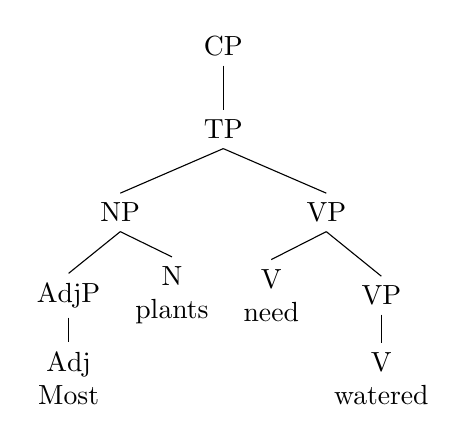
\begin{tikzpicture}
\Tree
[.CP
[.TP
	[.NP
		[.AdjP Adj\\Most ]
		N\\plants
	]
	[.VP V\\need
		[.VP V\\watered ]
	]
]
]

\end{tikzpicture}

\end{enumerate}

% question 2
\item Hixkaryana

% three parts
\begin{enumerate}

\item 

\begin{itemize}

\item NP $\rightarrow$ N (AdjP) (D)
\item VP $\rightarrow$ (NP) V
\item TP $\rightarrow$ VP NP

\end{itemize}

\item The order, both of constituents in a sentence and words in a phrase, generally appears to be the inverse of English.

\item \leavevmode\vadjust{\vspace{-\baselineskip}}\newline
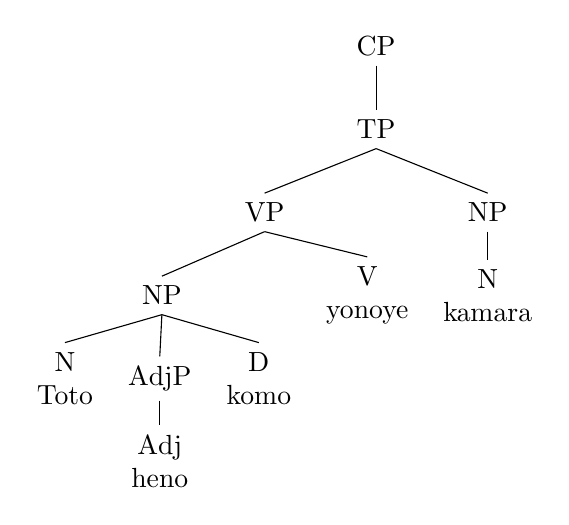
\begin{tikzpicture}
\Tree
[.CP
[.TP
	[.VP		
		[.NP N\\Toto
			[.AdjP Adj\\heno ]
		D\\komo ]
		V\\yonoye
	]
	[.NP N\\kamara ]
]
]

\end{tikzpicture}


\end{enumerate}

% question 3
\item Irish

\begin{enumerate}

\item NP $\rightarrow$ (D) N (AdjP)

\item If all we wanted was to account for the strings of the Irish data (that is, we ignored our proposed universals of object and subject locus), we could propose the following rule to generate Irish VPs:

VP $\rightarrow$ V NP (NP)

However, this violates the rule that the sentence subject cannot be dominated by the VP. There is no way to write a VP rule within the capacities of our CFG model. The second rule of precedence, "A or a node dominating A sister precedes B or a node dominating B", demonstrates that the linear order of Verb - Subject - Object does not fit within our tree's generative capacity given that the subject NP has to share common dominance with the object NP if it precedes the object NP, requiring both to be under the scope of the VP.

\item For the sake of this analysis, I will consider the object NP to be outside of the scope of the VP.

TP $\rightarrow$ VP NP (NP)

\item \leavevmode\vadjust{\vspace{-\baselineskip}}\newline
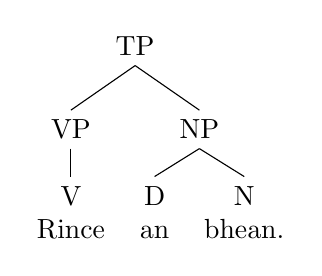
\begin{tikzpicture}
\Tree
[.TP
	[.VP V\\Rince ]
	[.NP D\\an N\\bhean. ]
]


\end{tikzpicture}

\end{enumerate}

% question 4
\item Argumentation

The following string (a) appears within the scope of the VP in sentence (b)

\begin{enumerate}
\item ``Barbie and Ken kissing''
\item Everyone at the party saw \textbf{Barbie and Ken kissing.}
\suspend{enumerate}

Our CFG model cannot predict whether this string is a constituent, given that it does not yet account for the syntactic behavior of participles (or many other non-finite verb forms, as discussed in question 1). However, I argue that various tests of constituency suggest that this string should be analyzed as a constituent, which can provide insight into how we can model the syntactic behavior of participles.

Rendering this sentence in the passive voice (all else being equal) dislocates the NP ``Barbie and Ken'' from the participle ``kissing.''

\resume{enumerate}
\item \textbf{Barbie and Ken} were seen by everyone at the party \textbf{kissing.}
\suspend{enumerate}

This dislocation does not necessarily prevent string (a) from being analyzed as a single constituent. Given that ``Barbie and Ken'' is unambiguously a constituent (our grammar predicts that it is a conjoined noun phrase), we can expect that a complex movement process like passivization might target it while leaving an element more peripheral to the overall node (here ``kissing'') behind in its original locus.

I will argue that, even with the passive syntax that generated this dislocation, various constituent tests prove that the words contained in string (a) are capable of behaving as a unit.

The string passes a simple replacement test.

\resume{enumerate}
\item \textbf{Barbie} was seen by everyone at the party.
\suspend{enumerate}

But this is a bad test given that the proposed constituent is not merely \textit{Barbie and Ken}, but rather, the event of them kissing. Replacing the whole constituent with just \emph{Barbie} removes the verbal meaning. A standalone test preserves this semantic quality.

\resume{enumerate}
\item \textbf{What} was seen at the party?

	- \textbf{Barbie and Ken kissing.}
\suspend{enumerate}

The fact that the neuter interrogative pronoun \emph{what} is needed instead of the personal \emph{who} demonstrates that ``Barbie and Ken kissing'' has a different semantic structure than just ``Ken and Barbie,'' and the fact that it can stand alone as the response to a question suggests constituency.

The words can also be placed into an \emph{it}-cleft.

\resume{enumerate}
\item It was \textbf{Barbie and Ken kissing} that was seen at the party.
\suspend{enumerate}

The alternation in agreement morphology on the copula (``were'' became ``was'') could point to constituency. In sentence (c) the agreement was marked as plural, likely because the [+plural] parameter was taken from the NP ``Barbie and Ken.'' If we assume that ``Barbie and Ken kissing'' is a itself also a constituent which contains ``Barbie and Ken,'' then we would expect the agreement parameter it passes to be different since, as stated above, its semantic structure is different than ``Barbie and Ken.''

Finally, the proposed constituent passes the reverse \emph{wh-}cleft test.

\resume{enumerate}
\item \textbf{Barbie and Ken kissing} is what was seen at the party.
\suspend{enumerate}

As stated above, our in its current state cannot draw any constituent tree for string (a). However, nor can it draw a string that incorporates ``kissing'' into any other phrase. In sentence (c), if we tried to associate it with the VP, we would have to place it after the head V - but our rule only allows for a single V in a VP, and ``kissing'' cannot belong to a CP since there is no full clause following the verb ``seen.''

Thus, I propose a rule similar to that in 1b. I add V as an alternative in the argument {CP/PP}+ in the NP rule, as below:

NP $\rightarrow$ ({NP Poss/D}) (AdjP+) N ({PP/CP/V}+)

Here V is specifically certain non-finite verbs that behave similarly to CPs, only that, in being non-finite, lack an overt subject and refer instead lean on a preceding NP in its binding domain as the semantic subject.

This hypothesis parsimoniously explains how string (a) can pass all the constituent tests applied above by extending an existent rule of our grammar (that CPs can occur at the end of NPs) to a similar structure (non-finite verbs like the participle ``kissing.'')

% question 5
\item Indogerman (Germesian?)

\begin{enumerate}

\item Indonesian can also form polar questions by moving the verb to the front of the sentence and adding the suffix \textit{-kah} to it.

\item In sentences (7a,b) \textit{apa} appears in the locus of the sentence where the direct object occurs, suggesting that it is functioning as the direct object of \textit{makan} and \textit{minum} respectively. In sentences (7c,d), \textit{apa} appears to have scope over the entire sentence and marks it as a polar question.

\item The polar question strategy presented in this assignment is similar to that of English, given that it involves moving an element to the front of the sentence. However, where English moves the T argument of the sentential TP, Indonesian moves the V argument.

\textit{Wh-}questions in Indonesian are different in English in that the \textit{wh}-element remains in situ, whereas in English it is moved to the front of the sentence.

\end{enumerate}


\end{enumerate}


\end{document}
